% Exam Template for UMTYMP and Math Department courses
%
% Using Philip Hirschhorn's exam.cls: http://www-math.mit.edu/~psh/#ExamCls
%
% run pdflatex on a finished exam at least three times to do the grading table on front page.
%
%%%%%%%%%%%%%%%%%%%%%%%%%%%%%%%%%%%%%%%%%%%%%%%%%%%%%%%%%%%%%%%%%%%%%%%%%%%%%%%%%%%%%%%%%%%%%%

% These lines can probably stay unchanged, although you can remove the last
% two packages if you're not making pictures with tikz.
\documentclass[11pt]{exam}
\RequirePackage{amssymb, amsfonts, amsmath, latexsym, verbatim, xspace, setspace}
\RequirePackage{tikz, pgflibraryplotmarks}

% By default LaTeX uses large margins.  This doesn't work well on exams; problems
% end up in the "middle" of the page, reducing the amount of space for students
% to work on them.
\usepackage[margin=1in]{geometry}
\usepackage{changepage}


% Here's where you edit the Class, Exam, Date, etc.
\newcommand{\class}{Principles of Operating Systems}
\newcommand{\term}{Spring 2017}
\newcommand{\examnum}{Midterm}
\newcommand{\examdate}{02/13/2017}
\newcommand{\timelimit}{9:00am - 9:50am}

% For an exam, single spacing is most appropriate
\singlespacing
% \onehalfspacing
% \doublespacing

% For an exam, we generally want to turn off paragraph indentation
\parindent 0ex

\begin{document} 

% These commands set up the running header on the top of the exam pages
\pagestyle{head}
\firstpageheader{}{}{}
\runningheader{\class}{\examnum\ - Page \thepage\ of \numpages}{\examdate}
\runningheadrule

\begin{flushright}
\begin{tabular}{p{2.8in} r l}
\textbf{\class} & \textbf{Name (Print):} & \makebox[2in]{\hrulefill}\\
\textbf{\term} &&\\
\textbf{\examnum} &&\\
\textbf{\examdate} &&\\
\textbf{Time Limit: \timelimit} & & \\
\end{tabular}\\
\end{flushright}
\rule[1ex]{\textwidth}{.1pt}




%\begin{minipage}[t]{3.7in}
%\vspace{0pt}
\begin{itemize}

\item \textbf{Don't forget to write your name on this exam.} 

\item \textbf{This is an open book, open notes exam. But no online or 
    in-class chatting.  } 

    
\item \textbf{Ask me if something is not clear in the questions.}

\item \textbf{Organize your work}, in a reasonably neat and coherent way, in
the space provided. Work scattered all over the page without a clear ordering will 
receive very little credit.  

\item \textbf{Mysterious or unsupported answers will not receive full
credit}.  A correct answer, unsupported by explanation will receive no credit; 
an incorrect answer supported by substantially correct explanations might still 
receive partial credit.

\item If you need more space, use the back of the pages; clearly indicate when you have done this.
\end{itemize}

%Do not write in the table to the right.
%\end{minipage}
%\hfill

%\begin{minipage}[t]{2.3in}
%\vspace{0pt}
%\cellwidth{3em}
%\gradetablestretch{2}
\vqword{Problem}
\addpoints % required here by exam.cls, even though questions haven't started yet.	
\gradetable[v]%[pages]  % Use [pages] to have grading table by page instead of question

%\end{minipage}
\newpage % End of cover page

%%%%%%%%%%%%%%%%%%%%%%%%%%%%%%%%%%%%%%%%%%%%%%%%%%%%%%%%%%%%%%%%%%%%%%%%%%%%%%%%%%%%%
%
% See http://www-math.mit.edu/~psh/#ExamCls for full documentation, but the questions
% below give an idea of how to write questions [with parts] and have the points
% tracked automatically on the cover page.
%
%
%%%%%%%%%%%%%%%%%%%%%%%%%%%%%%%%%%%%%%%%%%%%%%%%%%%%%%%%%%%%%%%%%%%%%%%%%%%%%%%%%%%%%

\begin{questions}

% Basic question
\addpoints
\question Basic page tables.


\begin{parts}
\part[5] 

Illustrate organization of the x86, 4K, 32bit 2-level page tables through an 
simple example. Assume that the hardware translates the virtual address
'0xc04005' (binary 0b1100 0000 0100 0000 0000 0101) into the physical address
'0x55005'.  The physical addresses of the page table directory and the page
table (Level 2) involved in the translation of this virtual address are 0x8000
and 0x2000. Draw a diagram, provide a short explanation. 

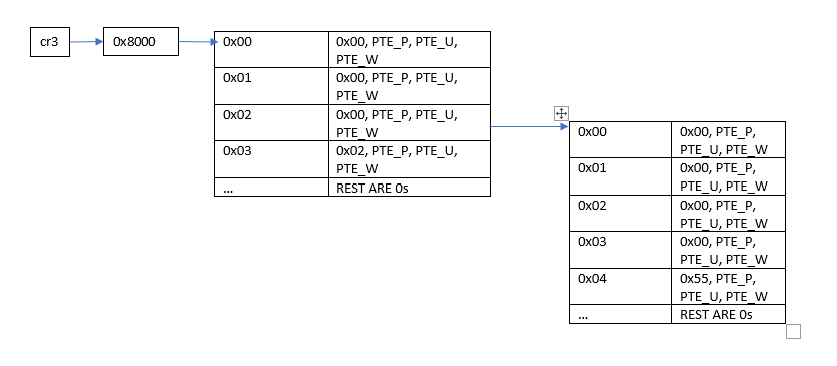
\includegraphics[width=0.8\columnwidth]{figs/1a-answ}

Idea -- we go find the location via the virtual addr, until the PT value, and give that PT value the correct offset to the desired phys page (in this case, 0x55000) and pass as the page table value.
\vfill 


%\part[10] Imagine you want to construct a two-level page table but have only
%one 4K physical page for both page table directory, and all level 2 page
%tables. What kind of address spaces you will be able to consrtuct?  Draw a
%picture, provide some discussion.

\vfill
\end{parts}

\newpage \addpoints

\question Xv6 shell implements a pipe command (e.g., ls | wc) as follows: 
\begin{verbatim}
8650 case PIPE:
8651 pcmd = (struct pipecmd*)cmd;
8652 if(pipe(p) < 0)
8653   panic("pipe");
8654 if(fork1() == 0){
8655   close(1);
8656   dup(p[1]);
8657   close(p[0]);
8658   close(p[1]);
8659   runcmd(pcmd->left);
8660 }
8661 if(fork1() == 0){
8662   close(0);
8663   dup(p[0]);
8664   close(p[0]);
8665   close(p[1]);
8666   runcmd(pcmd->right);
8667 }
8668 close(p[0]);
8669 close(p[1]);
8670 wait();
8671 wait();
8672 break;
\end{verbatim}

\begin{parts} 

\part[5] Why does the child process that runs the left-side of the pipe close
file descriptor 1 and why does the child process that runs the right-side of
the pipe close file descriptor 0?

\textbf{STUDENT SOLUTION } 
\begin{adjustwidth}{1.5em}{1em}
The file descriptor 1 is the standard output. So the left side process is the input of the pipe. It closes its standard output so that in the next dup command will copy the "input" end of the pipe, and direct all std out to the pipe.  
  
Likewise, the file descriptor 0 is the standard input So the right side process is the output of the pipe. It closes its standard input so that in the next dup command, the output of the pipe can be directed to the input of this process.
\end{adjustwidth}
\vfill

\part[5] It looks that in the sh.c code above after the first fork() (at line
8654) both parent and child will reach the second fork() (line 8661) creating
two child processes. Both child processes will start reading from the pipe and
will try to execute the right side of the pipe. This seems wrong. Can you
explain what is happening? 

\textbf{STUDENT SOLUTION } 
\begin{adjustwidth}{1.5em}{1em}
This is not true because in the runcmd function, the process will be executing a new program and they will exit rather than returning to the following codes in this page.
\end{adjustwidth}
\vfill

\end{parts}

% Question with parts
\newpage
\addpoints 

\question OS isolation and protection

\begin{parts} 

\part[5] In xv6 user processes cannot access kernel memory.  Explain why.   

\textbf{STUDENT SOLUTION } 
\begin{adjustwidth}{1.5em}{1em}
The U/S bit is not set in either page directory entry or page table entry (or both) for all translations that are allocated to kernel. Therefore, if a user tries to access this "kernel" memory, the page fault exception is raised after the bit is chekced by hardware.
\end{adjustwidth}
\vfill

\part[5] Imagine you have hardware that is identical to x86, but does not have
a user bit in the page tables. What changes need to be made to xv6 to ensure
isolation of the kernel from user-processes? 

\textbf{STUDENT SOLUTION } 
\begin{adjustwidth}{1.5em}{1em}
You could create an entirely seperate, new process so that whenver the kernel permissions are needed, one needs to process switch to kernel's process, therefore creating isolation.
\end{adjustwidth}
\vfill 

\end{parts} 

\newpage 

\addpoints

\question OS organization.

Imagine you want to optimize xv6 to run a large
number of very small processes. A realistic example can be a web server that
implements a Facebook's login page---you have to isolate each user in its own
process, otherwise a single exploit from any user reveals accounts of all users
going through the login page, but at the same time each process is very small
(it just sends out a simple HTML page). Entire logic of such web server program
can fit in 2-3K of memory.
 

\begin{parts} 


\part[10] You start by analizing the overheads involved into creating a
process. How many pages of memory are allocated when xv6 creates a smallest
process? Count both user-level and kernel resources.

\textbf{STUDENT SOLUTION } 
\begin{adjustwidth}{1.5em}{1em}
Since the process is small, we assume each part of the user-level program can fit in one page.

For user-level: One for text, one for data, one for guard page, one for stack, and 1 for the Page table directory, 1 for the Page table. Totally at least 6 on the user's side.

For kernel-level: 0 ~ 224MB, and we know that a page maps 4MB of space, that is it needs 224MB/4MB pages. Also, one for kernel stack, seven for BIOS region.

224 / 4 + 6 + 7 + 1
= 70

Therefore, in total there should be 70 pages.
\end{adjustwidth}
\vfill

\part[10] Suggest a set of changes to xv6 aimed at minimizing the number of
pages that are required for creating very small processes, e.g., the once that
are 1K in size.

\textbf{STUDENT SOLUTION } 
\begin{adjustwidth}{1.5em}{1em}
Carefully analyze what system calls are used by these web page processes. Then in the mapped kernel space, omit out the functions that are not used by these small programs. It should be common that the small programs should only use limited functions of the system - otherwise, they won't be small.

Another idea is that we could make a minimal kernel, where kernels are not mapped per process, so that each process would not need to map the entire kernel space.

\end{adjustwidth}

\vfill \end{parts}

\iffalse

\newpage
\addpoints
\question You are given a task of porting xv6 on the hardware that is identical 
to x86, but does not have a paging mechanism. 

\begin{parts}
\part[10] How will you implement address spaces? Remember that address spaces 
provide two key properties: illusion of a private memory, and isolation. Draw a 
figure of an address space layout for 2 processes and the kernel. Provide 
discussion of the mechanisms involved into your implementation.  

\vfill
\part[10] Remember that user processes on xv6 have only one interface to change 
their memory allocation---the \texttt{sbrk(n)} system call that allows the 
process to change its memory allocation growing it by n bytes (or shrinking it 
if a negative value is provided). How will you support \texttt{sbrk()} in your 
xv6 port? What are the data structures required? Provide a design discussion. 

\vfill
\newpage
\part[10] What if two processes want to share a region of memory? Can you 
suggest an interface and implementation for your port? What are the limitations 
of this mechanism, e.g. how many processes can share a region of memory 
simultaneously, how many sharing regions can be established? 

\vfill
\part[10] Discuss advantages and disadvantages of giving up the paging 
mechanism. 


\vfill
\end{parts}

\fi

% If you want the total number of points for a question displayed at the top,
% as well as the number of points for each part, then you must turn off the point-counter
% or they will be double counted.
%\newpage
%\addpoints
%\question[10] Even more work.
%\noaddpoints % If you remove this line, the grading table will show 20 points 
%for this problem.
%\begin{parts} \part[5] Even more...  \vspace{4.5in} \part[5] That's clearly
%too much \end{parts}



\end{questions}
\end{document}
